% $Id: Array_desc.tex,v 1.4 2004/04/22 16:28:11 nscollins Exp $

%\subsection{Description}

An ESMF Array, as one might expect, represents a multidimensional array.
It can be real, integer, or logical, and can possess up to seven 
dimensions.  The array can be strided.  The first dimension specified 
is always the one which varies fastest in linearized memory. 

Arrays can be created, destroyed, copied, and indexed.  Communication
methods, such as redistribution, are also defined.

\subsubsection{Array Halo Domains}

Array objects can have an optional {\bf halo width} which defines
what part of the array is the {\bf exclusive domain}, the {\bf computational
domain}, and the {\bf total domain}.  With no halo region, all these are
the same and equal to the total size of the array.  The domains are
defined as follows.

\begin{itemize}

\item {\bf Exclusive}  The exclusive domain is the subset of the
array which is never read by any other DE.  

\item {\bf Computational}  The computational domain
is the subset of the array which is read and written by the current DE.

\item {\bf Total}  The total domain is the entire array, which can 
contain regions where data is updated from another DE during a 
halo operation and read but not updated by the current DE.  

\end{itemize}

Figure \ref{fig:halo} illustrates these concepts.

Halo domain information must be stored at the Array level to
support operations such as the Gather operation which collects
decomposed parts of a logically contiguous object onto a single DE.
Only the computational domain is copied since the halo regions are
duplicated data.  The exclusive domain is guaranteed to never be
the source of data for a halo operation, so no synchronization
of updates to those data items needs to be done.  The total
domain is the actual memory size allocated for the array,
and is used when computing offsets for subdomains within the array.

\begin{center}
\begin{figure}
\caption{Diagram showing how ESMF exclusive, computational,
and total domains are defined.  }
\label{fig:halo}
\scalebox{1.0}{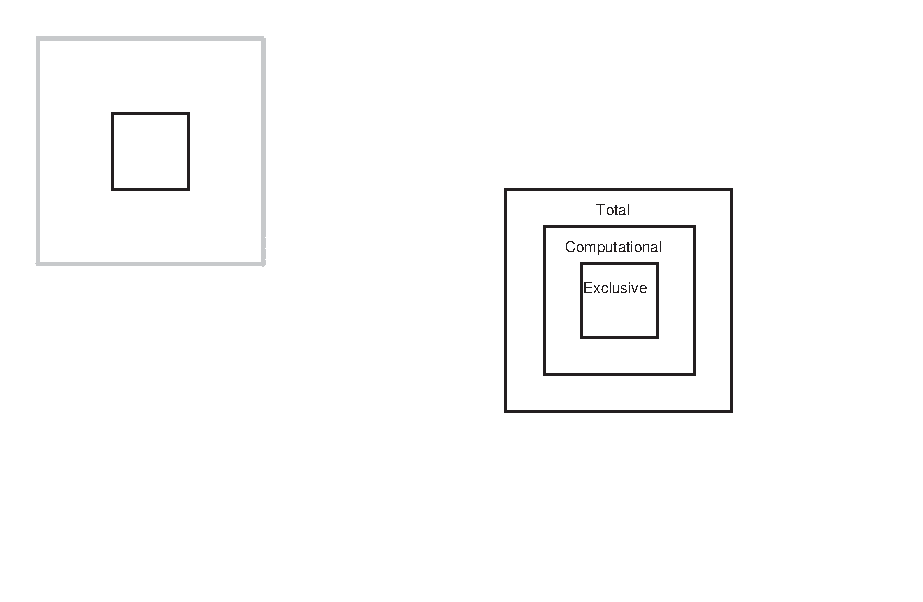
\includegraphics{Field_halo.eps}}
\end{figure}
\end{center}

